%Este trabalho está licenciado sob a Licença Creative Commons Atribuição-CompartilhaIgual 3.0 Não Adaptada. Para ver uma cópia desta licença, visite https://creativecommons.org/licenses/by-sa/3.0/ ou envie uma carta para Creative Commons, PO Box 1866, Mountain View, CA 94042, USA.

\chapter{Campos vetoriais}\label{cap:campos}\index{campos vetoriais}


\section{Campos escalares e campos vetoriais}
 Campo é termo usado para designar funções definidas em uma porção do espaço tridimensional (ou bidimensional), isto é, funções cujo domínio $D$ é um subconjunto de $\mathbb{R}^3$ (ou $\mathbb{R}^2$). Trabalharemos com dois tipos de campos: os campos escalares e os campos vetoriais. Os campos vetoriais são funções cuja imagem é composta de vetores no $\mathbb{R}^3$, já a imagem dos campos escalares são números reais, isto é, escalares.

\begin{ex}\label{excampos} São exemplos de campos escalares.
\begin{itemize}
\item [a)] A função que liga a posição de um ponto dentro de uma sala à temperatura neste ponto.
\item [b)] A pressão do ar como função da posição na atmosfera.
\item [c)] $f(x,y,z)= 100 + 20e^{-\sqrt{x^2+y^2+z^2}}$.
\item [d)] $f(x,y,z)= \vec{r} \cdot \vec{r} = x^2+y^2+z^2$, onde $\vec{r}=x\vec{i}+y\vec{j}+z\vec{k}$ .
\end{itemize}
\end{ex}


\begin{ex}\label{excampos} São exemplos de campos vetoriais.
\begin{itemize}
\item [a)] A função que liga a posição de um ponto dentro de uma fluido à velocidade (vetor) neste ponto.
\item [b)] O campo magnéticos, elétrico, gravitacional etc.
\item [c)] $\vec{F}(x,y,z)= x\vec{i} + z\vec{j} - y\vec{k}$.
\item [d)] $\vec{F}(x,y,z)= \vec{r}\times \vec{k}$
\end{itemize}
\end{ex}

\section{Representação gráfica dos campos vetoriais}
Um campo vetorial é representado graficamente por um conjunto de setas partindo de pontos $(x,y,z)$ e de comprimento proporcional ao módulo de $\vec{F}(x,y,z)$ e mesma direção e sentido de $\vec{F}(x,y,z)$. O conjunto de pontos é escolhido de forma arbitrária de forma a permitir interpretar o campo.

\begin{ex} Represente graficamente o campo vetorial $\vec{F}(x,y)=\sqrt{y}\ \!\vec{i},~~y\geq 0$.
%\begin{figure}[htp]
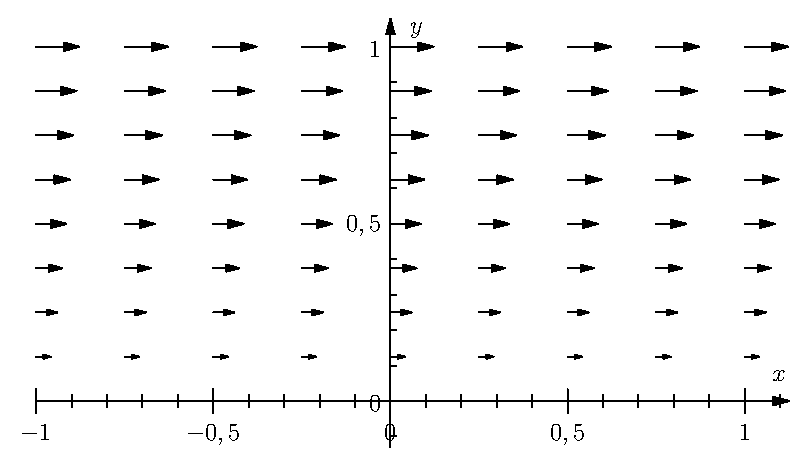
\includegraphics{cap_campos/figs/campo_exemplo_1}
%\caption{\label{campo_radial}Representação gráfica do campo $\vec{F}(x,y)=\sqrt{y}\ \!\vec{i},~~y\geq 0$.}
%\end{figure}
\end{ex}


\begin{ex} Represente graficamente o campo vetorial $\vec{F}(x,y)=x\vec{i},~~y\geq 0$.
%\begin{figure}[htp]
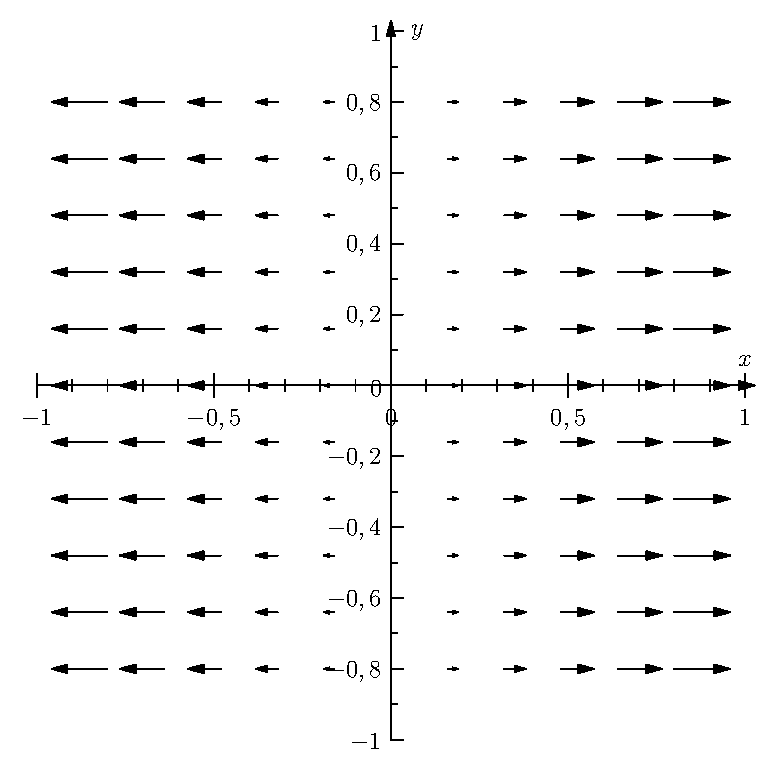
\includegraphics{cap_campos/figs/campo_exemplo_2}
%\caption{\label{campo_radial}Representação gráfica do campo $\vec{F}(x,y)=x\vec{i}$.}
%\end{figure}
\end{ex}

\begin{ex} Represente graficamente o campo vetorial $\vec{F}(x,y)=-y\vec{i}+x\vec{j}$.
%\begin{figure}[htp]
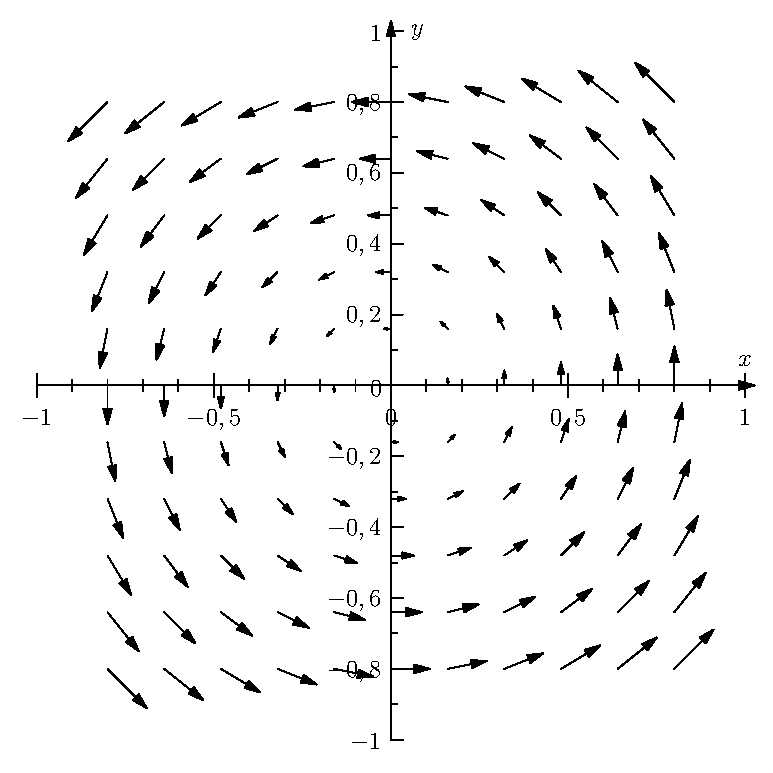
\includegraphics{cap_campos/figs/campo_exemplo_3}
%\caption{\label{campo_radial}Representação gráfica do campo $\vec{F}(x,y)=-y\vec{i}+x\vec{j}$.}
%\end{figure}
\end{ex}



\section{Cálculo com o operador nabla}
\subsection{Operador $\vec{\nabla}$}
No cálculo vetorial, o operador $\vec{\nabla}$, pronunciado nabla ou del, é um símbolo usado para denotar uma série de operadores diferenciais definidos em campos escalares e vetorias, como gradiente, divergente e rotacional. Ele é definido simbolicamente como:
\begin{equation}\label{def_del}
\vec{\nabla} \equiv \vec{i}\frac{\partial}{\partial x}+\vec{j}\frac{\partial}{\partial y}+\vec{k}\frac{\partial}{\partial z}
\end{equation}
Rigorosamente falando, o operador del não é um operador diferencial, mas um mnemônico que ajuda a lembrar de uma série de operadores diferenciais:
\begin{eqnarray*}
 \vec{\nabla}f &=& \vec{i}~\!\frac{\partial f}{\partial x}+\vec{j}~\!\frac{\partial f}{\partial y}+\vec{k}~\!\frac{\partial f}{\partial z} ~~ \text{(Gradiente)},\\
 \vec{\nabla}\cdot \vec{F} &=& \frac{\partial F_1}{\partial x}+\frac{\partial F_2}{\partial y}+\frac{\partial F_3}{\partial z} ~~ \text{(Divergente)},\\
 \vec{\nabla}\times \vec{F} &=&  \vec{i}\left(\frac{\partial F_3}{\partial y}-\frac{\partial F_2}{\partial z}\right) + \vec{j}\left(\frac{\partial F_1}{\partial z}-\frac{\partial F_3}{\partial x}\right) + \vec{k}\left(\frac{\partial F_2}{\partial x}-\frac{\partial F_1}{\partial y}\right)~~ \text{(Rotacional)}.\\
\end{eqnarray*}
O rotacional pode ser representado pelo seguinte determinante simbólico, que funciona como um mnemônico para lembrar facilmente de sua definição:
$$
 \vec{\nabla}\times \vec{F}=\left|
 \begin{array}{ccc}
 \vec{i} & \vec{j} & \vec{k} \\
 \frac{\partial}{\partial x} &\frac{\partial}{\partial y} &\frac{\partial}{\partial z} \\
F_1 & F_2 & F_3
 \end{array}
\right|.
$$

\begin{ex} Calule o gradiente do campo escalar dado por $f(x,y,z)=xy+z$.
\begin{eqnarray}
 \vec{\nabla}f &=& \vec{i}~\!\frac{\partial f}{\partial x}+\vec{j}~\!\frac{\partial f}{\partial y}+\vec{k}~\!\frac{\partial f}{\partial z}
 =y\vec{i}+x\vec{j}+\vec{k}
\end{eqnarray}
\end{ex}

\begin{ex} Calule o divergente e o rotacional do campo vetorial dado por $\vec{F}=(yz+x)\vec{i}+z^2\vec{j}+z^3\vec{k}$.
\begin{eqnarray}
 \vec{\nabla}\cdot \vec{F} &=& \frac{\partial F_1}{\partial x}+\frac{\partial F_2}{\partial y}+\frac{\partial F_3}{\partial z} =
 1+0+3z^2=3z^2+1
\end{eqnarray}

\begin{eqnarray}
  \vec{\nabla}\times \vec{F}&=&\left|
 \begin{array}{ccc}
 \vec{i} & \vec{j} & \vec{k} \\
 \frac{\partial}{\partial x} &\frac{\partial}{\partial y} &\frac{\partial}{\partial z} \\
yz+x & z^2 & z^3
 \end{array}
\right|\\&=&\left(0-2z\right)\vec{i}+\left(y-0\right)\vec{j}+\left(0-z\right)\vec{k}\\
&=&-2z\vec{i}+y\vec{j}-z\vec{k}.
\end{eqnarray}
\end{ex}

\begin{ex} Dado o campo vetorial dado por $\vec{F}=x^5\vec{i}+y^2\vec{j}$, calcule o gradiente do divergente,$ \vec{\nabla} \vec{\nabla}\cdot \vec{F}$, de $\vec{F}$
\begin{eqnarray}
 \vec{\nabla}\cdot \vec{F} &=& \frac{\partial F_1}{\partial x}+\frac{\partial F_2}{\partial y}+\frac{\partial F_3}{\partial z} =
 5x^4+2y\\
 \vec{\nabla} \vec{\nabla}\cdot \vec{F}&=&20x^3\vec{i}+2\vec{j}
\end{eqnarray}
 \end{ex}

\subsection{Operadores diferenciais de segunda ordem}
Operadores diferenciais de segunda ordem podem ser definidos através da composição de operadores diferenciais de segunda ordem. Combinando o gradiente, rotacional e divergente, encontramos as seguintes possibilidades:\index{operador!de segunda ordem}\index{operador!laplaciano}
\begin{eqnarray}
  \vec{\nabla} \cdot \vec{\nabla} f&~& \text{(Divergente do gradiente ou laplaciano)}\\
  \vec{\nabla} \times \vec{\nabla} f&~& \text{(Rotacional do gradiente)}\\
  \vec{\nabla} \vec{\nabla}\cdot \vec{F}&~& \text{(Gradiente do divergente)}\\
  \vec{\nabla} \cdot{\nabla}\times \vec{F}&~& \text{(Divergente do rotacional)}\\
  \vec{\nabla} \times{\nabla}\times \vec{F}&~& \text{(Rotacional do rotacional)}\\
  \end{eqnarray}
Os operadores $\vec{\nabla} \times \vec{\nabla}$ e $\vec{\nabla} \cdot{\nabla}\times \vec{F}$ são identicamente nulos, o que pode ser provado por simples inspeção
\begin{eqnarray}
 \vec{\nabla} \times \vec{\nabla} f &=&\left|
 \begin{array}{ccc}
 \vec{i} & \vec{j} & \vec{k} \\
 \frac{\partial}{\partial x} &\frac{\partial}{\partial y} &\frac{\partial}{\partial z} \\
\frac{\partial f}{\partial x} & \frac{\partial f}{\partial y} & \frac{\partial f}{\partial z}
 \end{array}
\right|\\
&=&\vec{i}\left(\frac{\partial^2 f }{\partial z\partial y} - \frac{\partial^2 f}{\partial y\partial z}\right) + \vec{j}\left(\frac{\partial^2 f}{\partial  x\partial z}-\frac{\partial^2f}{\partial z\partial x}\right) + \vec{k}\left(\frac{\partial^2 f}{\partial y\partial x}-\frac{\partial^2 f}{\partial x\partial y}\right)
\end{eqnarray}
Sob sufiente regularidade, as derivadas parciais podem ser comutadas e cada termo do rotacional é nulo, isto é:
\begin{eqnarray}
 \vec{\nabla} \times \vec{\nabla} f &\equiv &0
\end{eqnarray}
 para todo $f$ continuamente diferenciável.

\subsection{Derivada direcional e gradiente}
\subsection{Divergente}
\subsection{Rotacional}
\section{Identidades envolvendo o operador nabla}
\begin{equation}\label{rot_grad}
\vec{\nabla}\times\vec{\nabla}f=\vec{0}
\end{equation}


\section{Campos conservativos}
\begin{defn} \label{def_campo_conservativo}\index{campo!conservativo}\index{campo!rotacional}\index{campo!gradiente}  Um campo $\vec{F}(x,y,z)$ é dito conservativo se existe um campo escalar $\varphi(x,y,z)$ tal que
$$\vec{F}(x,y,z) = \vec{\nabla}\varphi$$
Neste caso $\varphi$ é chamado de campo potencial de $$\vec{F}(x,y,z)$$
\end{defn}
\begin{obs} Campos conservativos também são conhecidos como campos grandiente ou campos irrotacionais, este último nome advém do fato que $$\vec{\nabla}\times\vec{F}(x,y,z) = \vec{\nabla}\times\vec{\nabla}\varphi=\vec{0}.$$
Esta identidade é oriunda da Equação~\ref{rot_grad}.
 \end{obs}
\begin{ex} O campo $\vec{F}=2xy\vec{i}+x^2\vec{j}$ é conservativo por $\vec{F}=\vec{\nabla}\left(x^2y\right)$.
 \end{ex}

\begin{teo} Seja $\vec{F}:\mathbb{R}^3\to\mathbb{R}^3$ um campo vetorial contínuo e $\vec{\nabla}\times \vec{F}=\vec{0}$, então $\vec{F}$ é conservativo.
 \end{teo}
\begin{proof} Como $\vec{\nabla}\times \vec{F}=\vec{0}$, temos:
\begin{eqnarray}
 \frac{\partial F_3}{\partial y} &=&\frac{\partial F_2}{\partial z}\label{rot_zero_x},\\
 \frac{\partial F_1}{\partial z} &=&\frac{\partial F_3}{\partial x}\label{rot_zero_y},\\
 \frac{\partial F_3}{\partial x} &=&\frac{\partial F_1}{\partial y}\label{rot_zero_z}.
\end{eqnarray}
Defina, agora, a função $\varphi:\mathbb{R}^3\to\mathbb{R}$ dada por
$$\varphi(x,y,z)=\int_0^xF_1(s,y,z) + \int_0^yF_2(0,s,z)+\int_0^zF_3(0,0,s).$$
Basta provar que $\vec{\nabla}\varphi(x,y,z)=\vec{F}$, isto é
\begin{eqnarray}
 \frac{\partial \varphi}{\partial z} &=&F_1,\label{rot_zero_der_x}\\
 \frac{\partial \varphi}{\partial y} &=&F_2,\label{rot_zero_der_y}\\
 \frac{\partial \varphi}{\partial z} &=&F_3\label{rot_zero_der_z}.
\end{eqnarray}
A primeira desigualdade advém diretamente do teorema fundamental do cálculo. Para obter a segunda desigualdade, derivamos o potencial em relação a $y$:
\begin{eqnarray*}
\frac{\partial }{\partial y}\varphi(x,y,z)&=&\int\int 0^x \frac{\partial }{\partial y}F_1(s,y,z)ds+ F_2(0,y,z)\\
&=&\int_0^x \frac{\partial }{\partial s}F_2(s,y,z)ds+ F_2(0,y,z)\\
&=&\left(F_2(x,y,z)-F_2(0,y,z)\right)+ F_2(0,y,z) = F_2(x,y,z)
\end{eqnarray*}
Onde usamos a Identidade~\ref{rot_zero_y}.

Finalmente, para obter a terceira desigualdade, derivamos o potencial em relação a $z$:
\begin{eqnarray*}
\frac{\partial }{\partial z}\varphi(x,y,z)&=&\int_0^x \frac{\partial }{\partial z}F_1(s,y,z)ds + \int_0^y \frac{\partial }{\partial z}F_2(0,s,z)ds+F_3(0,0,z)\\
&=&\int_0^x \frac{\partial }{\partial s}F_3(s,y,z)ds + \int_0^z \frac{\partial }{\partial s}F_3(0,s,z)ds+F_3(0,0,z)\\
&=&\int_0^x \left(F_3(x,y,z)-F_3(0,y,z)\right) + \left(F_3(0,y,z)-F_3(0,0,z)\right)+F_3(0,0,z)\\
&=&F_3(x,y,z)\\
\end{eqnarray*}
  Onde usamos as Idendidade~\ref{rot_zero_x} e \ref{rot_zero_z}.
\end{proof}




\section{Campos radiais e potenciais centrais}
Campos radiais vetoriais \index{campos radiais} são campos da forma $\vec{F}=f(r) \hat{r}$, isto é campos vetoriais cujo módulo depende apenas da distância até a origem, isto é, de $r=\|\vec{r}\|=\sqrt{x^2+y^2+z^2}$ e cuja direção é sempre paralela ao vetor posição, $\vec{r}$.
\begin{ex} Represente graficamente o campo vetorial $\vec{F}=\vec{r}$ no plano $xy$.
%\begin{figure}[htp]
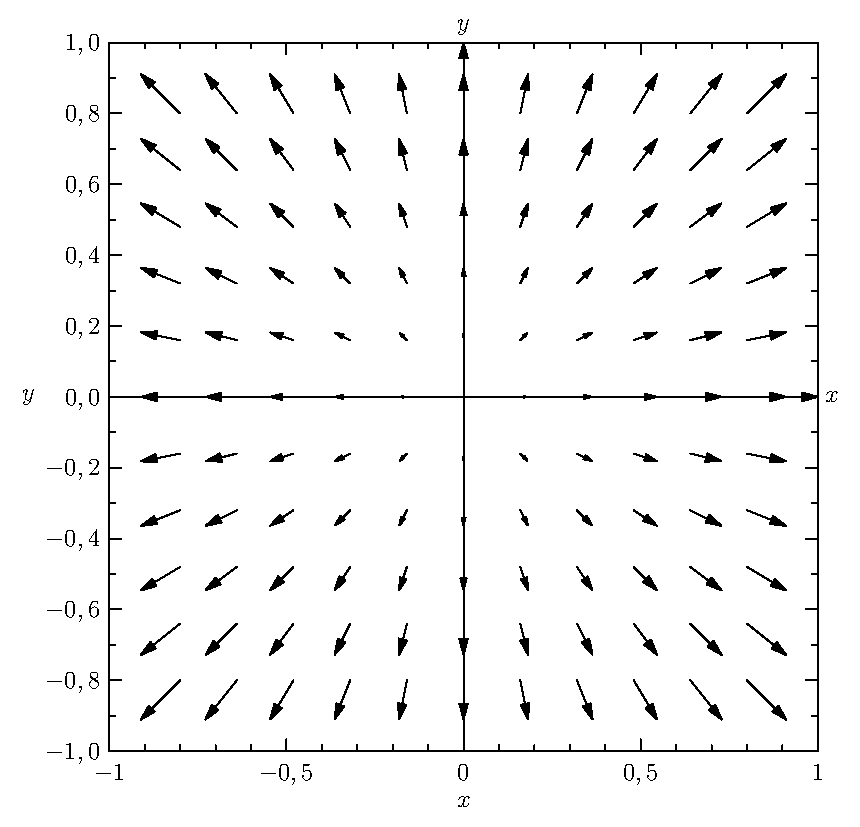
\includegraphics{cap_campos/figs/campo_radial}
%\caption{\label{campo_radial}Representação gráfica do campo $\vec{F}=\vec{r}$}
%\end{figure}
\end{ex}





\construirSec

\subsection*{Exercícios resolvidos}

\construirExeresol

\begin{exeresol}
  Um exercício.
\end{exeresol}
\begin{resol}
  Resolução do exercício.
\end{resol}

\subsection*{Exercícios}

\construirExer

\begin{exer}
  Um exercício.
\end{exer}
\begin{resp}
  Resposta curta do exercício.
\end{resp}

\section{Exercícios finais}

\construirExer

\begin{exer}
  Um exercício.
\end{exer}
\begin{resp}
  Resposta curta do exercício.
\end{resp}
